\section{Software Design} \label{sec:software}

As this experiment is deployed globally, it is imperative that the software stack be easy to build, install, and use, all with very little assistance from the project maintainers.
New members should be able to on-board their stations independently, just by following online documentation\urlfootnote{https://grex-telescope.github.io}.
As such, we developed the software stack for this instrument with intense attention to these goals.
As much as possible, software is tested in continuous integration and written in a way to reduce the likelihood of unexpected errors.
Additionally, all the software for the project is freely accessible and under an open-source license.

\subsection{Digitization and Initial Processing}

Following the analog signal path, the high-frequency signals are digitized by the Smart Network ADC Processor (SNAP)\urlfootnote{https://casper.berkeley.edu/wiki/SNAP} board.
This platform contains three HMCAD1511 analog to digital converters (ADC) from Analog Devices and a Kintex-7 160T field-programmable gate array (FPGA) from Xilinx.
This platform is supported by the CASPER~\cite{hickishDecadeDevelopingRadioAstronomy2016a} ecosystem, which we make use of here.

We wrote our gateware\urlfootnote{https://github.com/GReX-Telescope/gateware} in a combination of Simulink and SystemVerilog using the CASPER toolflow.
To make maximum use of the available 10G connection, we stream 8+8 bit complex data for each polarization, channelized to 2048 frequency bins.
As the FPGA core is clocked at 250 MHz, with the ADC clock running 500 MHz, the F-engine processes two ADC samples every clock cycle.
The channelization is accomplished with a standard polyphase filterbank constructed via the combination of a finite impulse response (FIR) filter and fast Fourier transform (FFT), both making use of design blocks from the CASPER library.
The FIR filter has 8 taps and a Hamming windowing function to reduce inter-channel leakage and scalloping loss~\cite{thompsonDigitalSignalProcessing2017}.
To avoid overflows in the FFT, each stage is allowed to grow the number of bits representing each channel.
The output of the FFT block is 18+18 bit, fixed-point complex numbers.
If we attempted to stream these data directly, we would not have the bandwidth on the 10G link.
As such, these data are requantized to a lower bit-depth of 8+8 bits to fit in a single 10G Ethernet payload.
Finally, the resulting channelized voltage data is packetized for transmission.
The block of data includes a 64-bit packet counter header, allowing the downstream software to detect data loss and re-ordering.
These data were packed such that they match the layout of a C-struct, so no processing needs to be done to use the data downstream.
The packetized data is transmitted over the optical 10G Ethernet link to the server, making use of the standard Ethernet block from CASPER.
Every 2048 samples, a completed Ethernet payload is transmitted, including the header, totalling 8200 bytes.
This occurs every 8.192 us, implying a total data rate of just over 1 GB/s or 8 GiB/s.

\begin{figure}[t!]
    \centering
    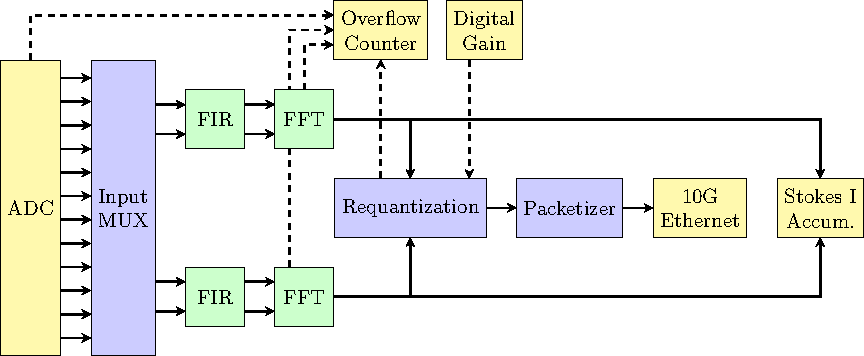
\includegraphics[width=\linewidth]{figures/gateware.pdf}
    \caption[FPGA gateware internals]{FPGA gateware internals: yellow blocks represent CASPER-provided interfaces to hardware, blue blocks are custom SystemVerilog, and green blocks are CASPER-provided DSP logic. Solid lines represent high-speed data, dashed lines represent slow monitor and control data. Reset lines and timing logic are not shown.}
    \label{fig:gateware}
\end{figure}

In addition to the primary functionality of the gateware, there are a few added utilities to assist in operation.
First, there is an input multiplexer that allows the user to connect to any input on the SNAP without reprogramming.
Second, there is a triggerable accumulator for Stokes I data that gives the user a snapshot view of the spectra without running high-speed packet capture.
Additionally, this accumulation is performed on the raw output from the FFT block, providing insight into the required digital gain setting for requantization.
Finally, there are various registers that monitor overflow conditions in both requatization, FFT bit growth, and raw ADC samples.
This primarily gives us an indication that the total power level into the SNAP board is too high, or downstream digital gain is too high, either case being actionable via the adjustable RF attentuators in the FEM or in the digital gain settings.
A figure of the data flow in the gateware is shown in \autoref{fig:gateware}.

\subsection{FPGA Software Interface}

A critical piece of code in the project is the software interface to the running FPGA gateware.
During telescope operation, status registers and accumulators are read, variables are set, etc.
For this project, we chose to write a new interface to CASPER devices using the Rust programming language, \textit{casperfpga\_rs}\urlfootnote{https://github.com/kiranshila/casperfpga_rs}.
The new library generates compile-time checked interfaces to the various components in the running FPGA design.
As the generated code fully validates correctness at compile-time, runtime errors are all but eliminated.

This new library allows for much higher confidence in the deployment of CASPER designs.
This library also contains unit tests against a mock interface, extensive documentation, and is written in a modular nature to encourage other members of the CASPER collaboration to add support for their hardware.

\subsection{Server and First Stage Processing} \label{subsec:t0}

After packets have been transmitted from the FPGA, they are captured and processed by a single high-performance server.
This server contains a 24-core AMD Ryzen Threadripper Pro 5965WX with 128 GB of RAM.
The server is also outfitted with an NVIDIA GeForce RTX 3090 Ti GPU, used for the brute-force dedispersion search.
This system's kernel parameters are tuned to support the “jumbo Ethernet frames” emitted from the SNAP board.
After the packets have been processed through the kernel, user-space programs perform the remaining processing.

The majority of the effort in software development for this project was in the first stage processing program, \textit{T0}.
This program performs the packet capture, computation of Stokes I, time downsampling, and management of ring buffers of voltage data to be written to disk on command.
As this piece of software handles the raw voltage data, it is the most timing sensitive and performance-critical.

At the top level, \textit{T0} consists of many independent threads, each performing a processing step called a subtask.
One thread is dedicated to the packet capture subtask, one for time-downsampling, etc.
We must use multithreading as the total processing time is longer than the incoming packet cadence, so parts of the processing need to be broken up and performed in parallel, i.e., pipelined.
After each subtask completes computation, it passes the result to the subsequent subtask across a thread boundary.

Our implementation of this streaming processing pipeline is built off the inter-process communication model of channels with allocation-reusing ring buffers, similar in spirit to PSRDADA~\cite{vanstratenPSRDADADistributedAcquisition2021}.
Unlike PSRDADA, the model is fully contained in a single executable, allowing for much stronger guarantees around the data being passed around.
Additionally, this model reduces the need for synchronization primitives such as mutexes, improving performance. 
\begin{figure}[t!]
    \centering
    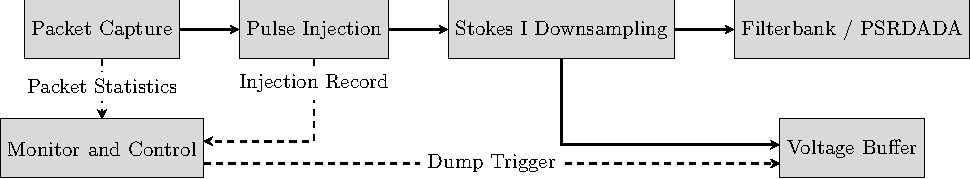
\includegraphics[width=\linewidth]{figures/t0.pdf}
    \caption[\textit{T0} subtasks and inter-thread communication]{\textit{T0} subtasks and inter-thread communication. Solid lines represent high-speed science data, dashed lines represent monitor and control.}
    \label{fig:t0_subtasks}
\end{figure}

The complete architecture of \textit{T0} is shown in \autoref{fig:t0_subtasks}, with arrows showing the channels that move data across the various threads.
After program start and timing synchronization (described in the \autoref{sec:timing}), all the subtasks are spawned simultaneously.
The first subtask again is packet capture, where incoming data is read from the network card.
This subtask checks the value of the packet header against the previous to test for packet loss or reordering.
Metadata about the packet statistics is transferred using a separate channel to the monitoring thread.
The following subtask performs fake pulse injection.
As we want to ensure our pipeline is working properly, we occasionally add synthetic data of various dispersion measures and fluence into the real-time data stream.
We write information about the injection into a \textit{SQLite} database, so downstream processing software can determine if a given candidate is synthetic.
The next subtask performs time downsampling.
Downstream processing, specifically brute-force dedispersion, has trouble handling exceptionally high time resolution data.
As such, we need to perform downsampling in time, in addition to computing Stokes I as we will be performing incoherent dedispersion.
Finally, depending on launch arguments, the downsampled Stokes I data is written to either a \textit{SIGPROC}\urlfootnote{https://sigproc.sourceforge.net/} filterbank file (using a high-performance Rust implementation\urlfootnote{https://github.com/kiranshila/sigproc_filterbank} of the file format) or to a \textit{PSRDADA}\urlfootnote{https://psrdada.sourceforge.net/} ring buffer.

Running in parallel to the data processing pipeline, a thread is accumulating and distributing monitor information.
This data includes occasional queries to the FPGA about overflow statistics, long-integration Stokes I spectra, and internal temperatures.
Moreover, it collects log messages produced by the program and statistics about packet capture from the first subtask.
The monitor subtask provides an HTTP API to query the monitor information for a Prometheus\urlfootnote{https://prometheus.io/} time-series database.
Log messages and traces are ingested by an \textit{OpenTelemetry}\urlfootnote{https://opentelemetry.io/} collector.

\subsection{Data Loss}
As the packets are transmitted over Ethernet with the UDP protocol, there is no guarantee that they are received.
We have taken special care to ensure the server's operating system can efficiently process incoming UDP data without data loss and \textit{T0} should be able to process incoming data in real time without issue.
However, packet loss still does occur, albeit rare.
For the Owens Valley station, the average packet loss rate is $10^{-6}$\% or one packet dropped per $10^8$ packets processed.
As our packet cadence is one packet per $8.192\,\mu\text{s}$, this works out to an average of one dropped packet per $1000\,\text{s}$.
This amount of data loss is to be expected and is inconsequential to the performance of the telescope.

\subsection{Timing and Synchronization} \label{sec:timing}
In the box, we include a GPS-discriminated $10\,\text{MHz}$ oscillator.
This device provides a stable reference and emits a pulse-per-second (PPS) square wave, connected to a general purpose digital input on the FPGA.
The $10\,\text{MHz}$ reference clock is used by a Valon 5009a frequency synthesizer to produce the $500\,\text{MHz}$ clock used by the ADC and FPGA.
Furthermore, this synthesizer is used to generate the $1030\,\text{MHz}$ local oscillator signal used in the FEM for downconversion.

In the FPGA gateware, the PPS signal is used to timestamp data.
In \textit{T0} at program start, we query a network timeserver to get the current local time within tens of milliseconds.
Then, the program waits until the next half second to ``arm'' the timing system on the FPGA.
Once the next rising edge of the PPS signal arrives in the FPGA and starts the flow of data, we know that the very first voltage sample is coincident with the next whole second.

As each packet has a 64 bit packet counter, and we know the timestamp of the first packet and know the clock speed of the FPGA, we can work out the start time of every packet.
Specifically, we know that packet $N$ is exactly $N\cdot8.192\,\mu\text{s}$ past the time of the first packet.
This information is used in the metadata stored in voltage dumps as well as in the candidate metadata.

\subsection{RFI Cleaning} \label{subsec:rfi_clean}

Following \textit{T0}, data is transferred to an RFI cleaning program, \textit{clean\_rfi}\urlfootnote{https://github.com/GReX-Telescope/clean_rfi} using \textit{PSRDADA} ring buffers.
This program implements a multistep cleaning approach following the implementation in CHIME/FRB~\cite{rafiei-ravandiMitigatingRadioFrequency2023}.

For both \textit{T0} and \textit{clean\_rfi}, we needed a Rust interface to the \textit{PSRDADA} C library, as that is the only mechanism to stream data into the brute-force dedispersion program, \textit{HEIMDALL}~\cite{barsdellAcceleratingIncoherentDedispersion2012}.
While Rust has a robust interface to C programs and libraries, they are all memory-unsafe by default, as there is no mechanism to guarantee Rust's invariants across the application binary interface (ABI) boundary.
As such, we wrote a high-level Rust wrapper library called \textit{psrdada\_rs}\urlfootnote{https://github.com/kiranshila/psrdada-rs}.
Much like \textit{casperfpga\_rs}, this library adds a significant number of compile-time checks to guarantee correct usage before runtime.

\textit{clean\_rfi} implements simple masking, variance-cut, and detrending algorithms to iteratively remove RFI from a block of dynamic spectra.
Specifically, we start with a static mask of bad channels for frequencies that are consistently contaminated.
Then, we remove all samples that contain zeros, as the typical noise floor will be just above zero and pure-zeros represent dropped packets.
Next, we remove bandpass variation by dividing each sample by the time-average frequency response.
Finally, we perform variance cuts in both the frequency and time axes by removing data above some $\sigma$ threshold.
We perform these final variance cuts twice, with a higher $\sigma$ in the second pass.
Currently, the iterative variance cut process removes time samples / frequency channels that are greater than $3\sigma$ and then $5\sigma$.

\subsection{Real-Time Detection Pipeline}\label{sec:realtime}

\begin{figure}[t!]
    \centering
    \parbox[t][][t]{.3\textwidth}{
        \centering
        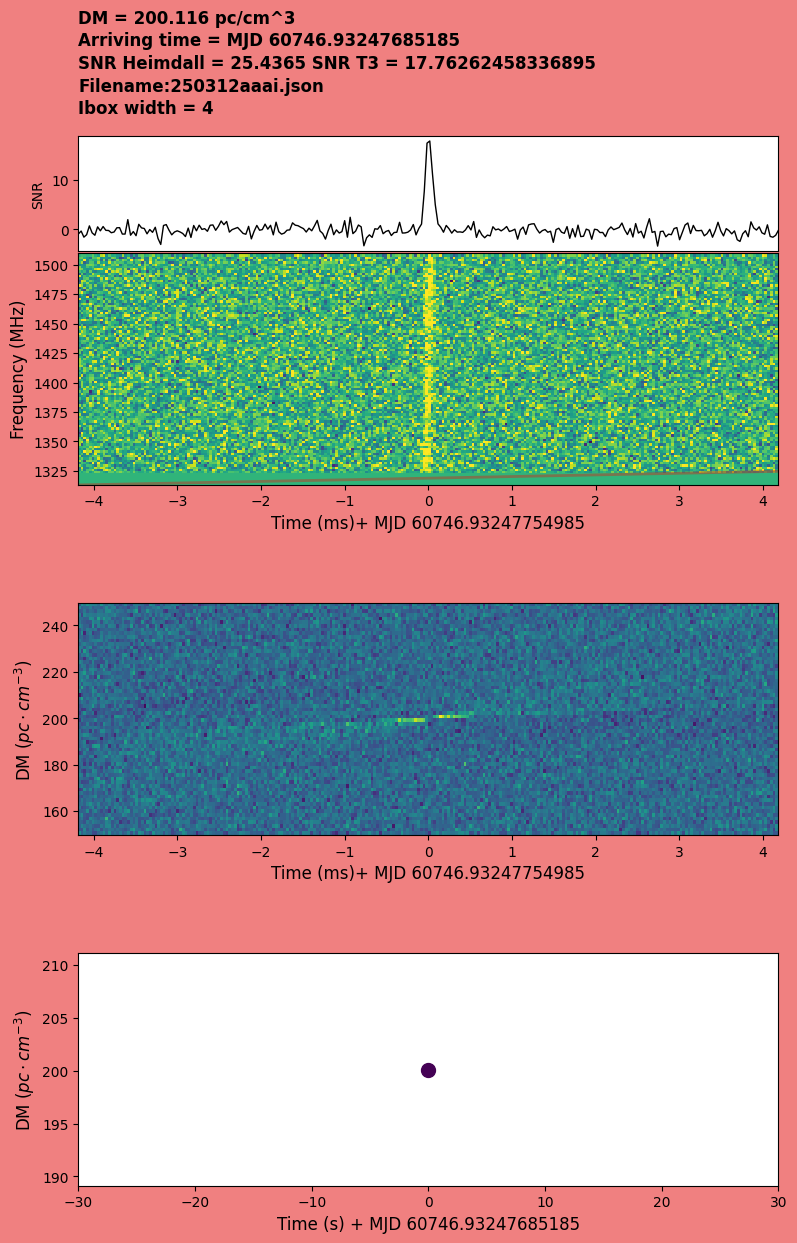
\includegraphics[height=5cm]{figures/injection_cand.png}
        \caption{Detection candidate for an injected burst}%
        \label{fig:injection_cand}
    }~
    \parbox[t][][t]{.65\textwidth}{
        \centering
        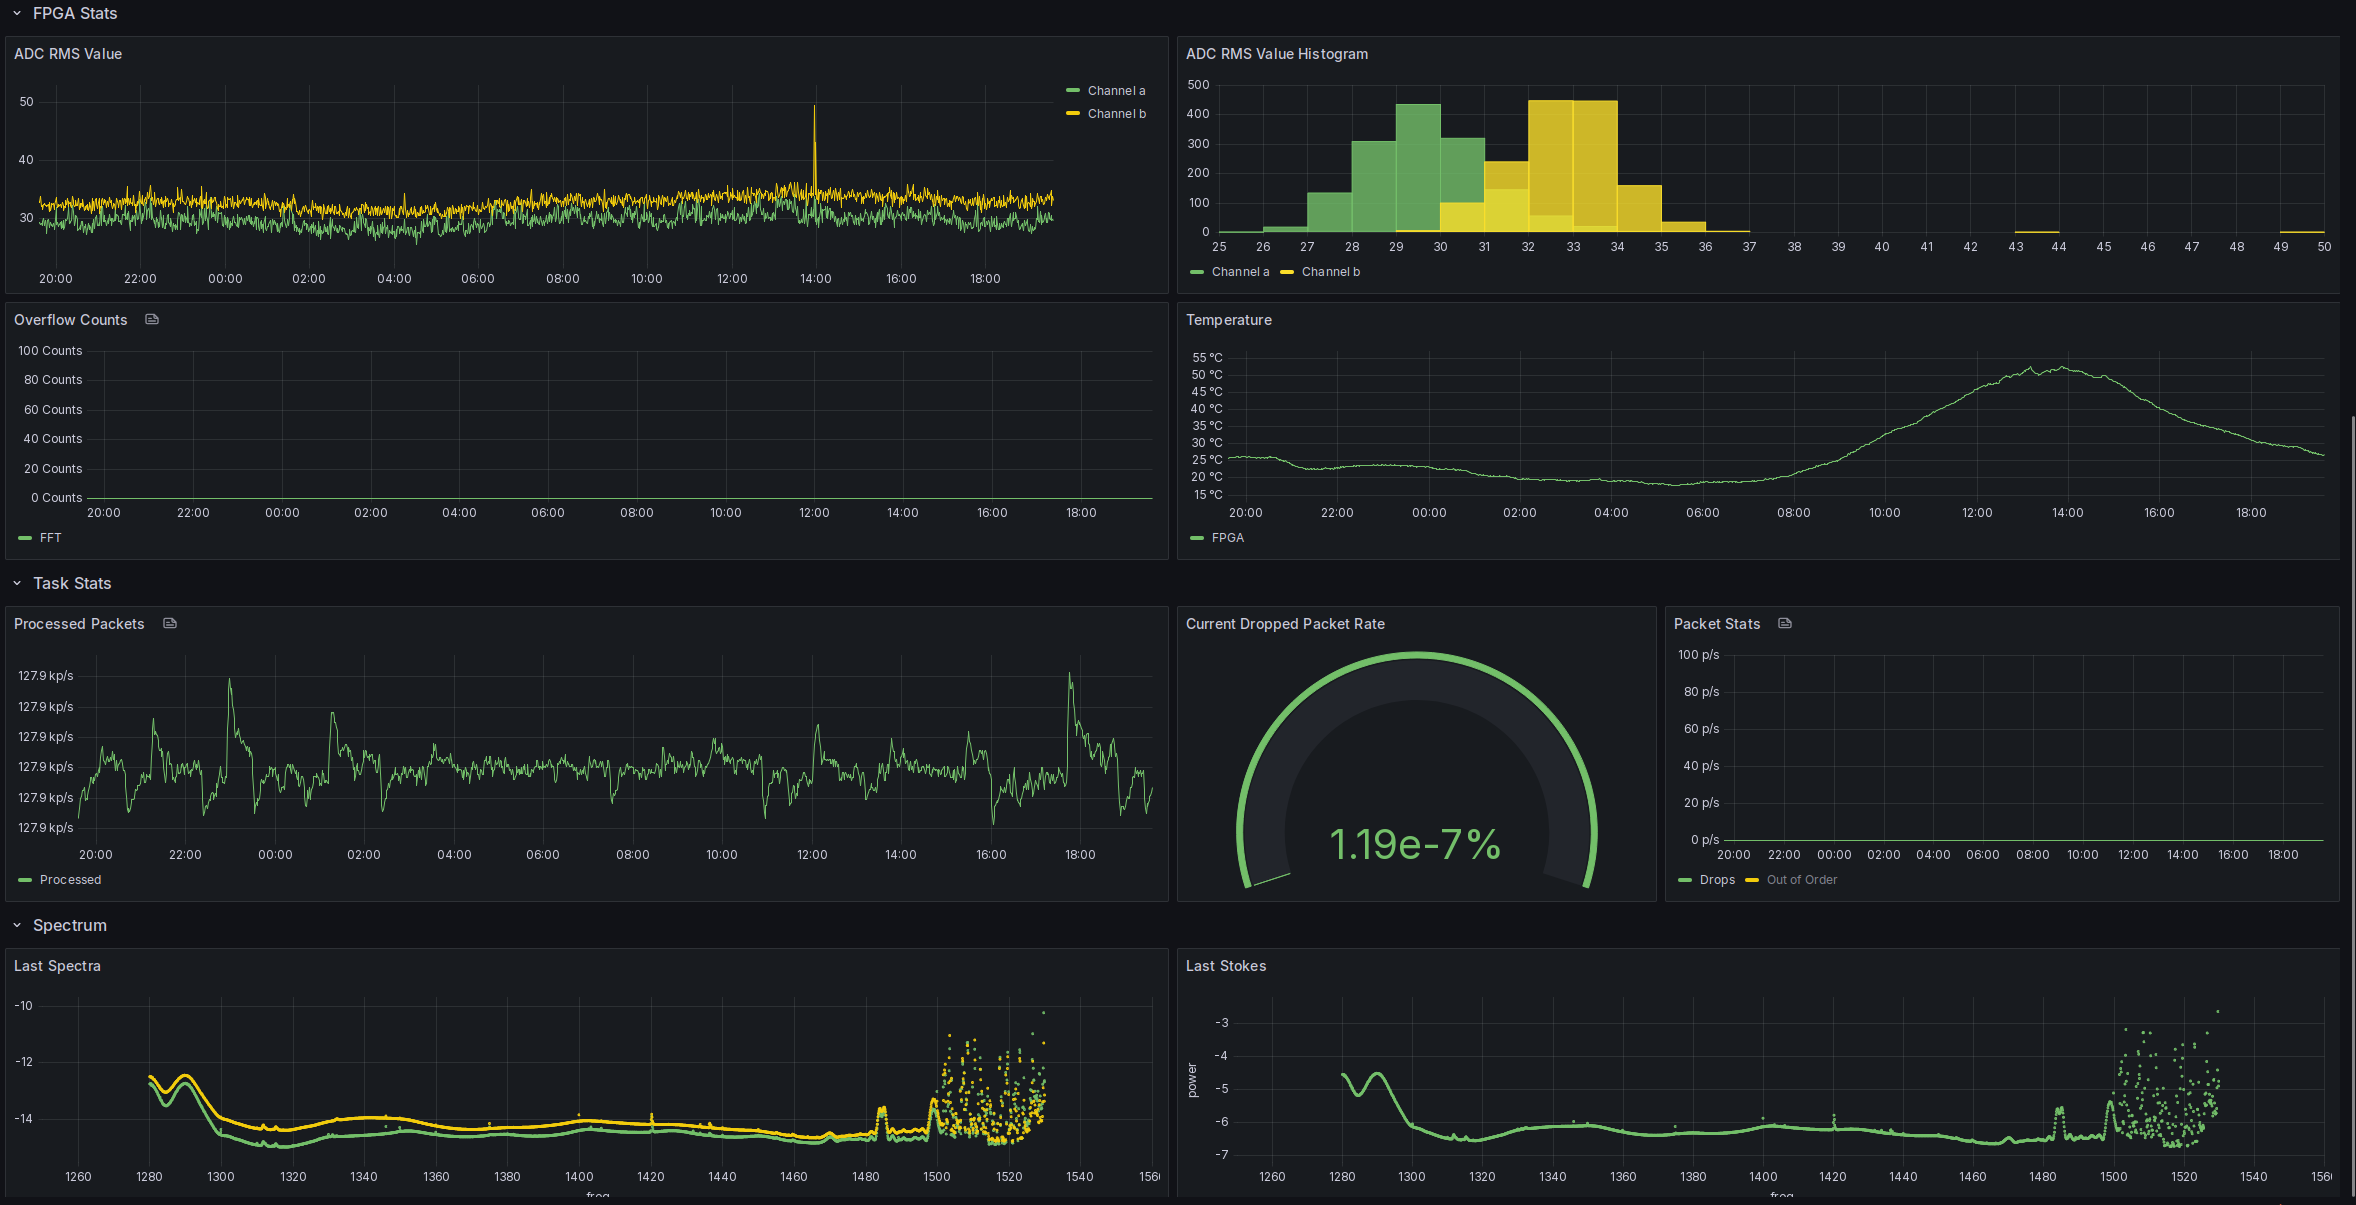
\includegraphics[height=4.5cm]{figures/grafana_ovro.png}
        \caption{Grafana dashboard monitoring system performance}%
        \label{fig:ovro-dash}
    }
\end{figure}

After the dynamic spectra data were cleaned, they are passed along to our fork\urlfootnote{https://github.com/GReX-Telescope/heimdall-astro} of HEIMDALL.
We use HEIMDALL, and the associated \textit{dedisp} library, as the implementation of the brute-force dedispersion search.
Our fork removes the built-in RFI cleaning routines, removes candidate clustering, adds a structured logging library, and enables writing candidates to a network socket instead of a file.
As we will be running the search in real time, the included RFI cleaning and clustering routines were too slow for our high time-resolution data.

HEIMDALL then writes lines of candidates over a local network socket to the candidate filtering task, \textit{T2}.
This program is a fork of the \textit{T2} Python project written for DSA-110, modified to work with our data formats.
This program ingests the stream of candidates emitted by HEIMDALL, clusters them using HDBSCAN~\cite{mcinnesHdbscanHierarchicalDensity2017}, filters the clustered results in dispersion measure, SNR, and boxcar width to produce candidates.
Additionally, for every viable candidate, a message is sent to \textit{T0} to dump the contents of the voltage ring buffer to disk.

\textit{T3} is the final stage in the pipeline, another fork from the DSA-110 project.
This program watches the directory where candidate files are written and generates plots of the dedispersed, RFI-cleaned dynamic spectra.
These candidate plots are then pushed to a Slack channel, where members of the collaboration get real-time notifications.
An example of this notification is shown in \autoref{fig:injection_cand}.
Eventually, \textit{T3} will perform machine learning-based candidate classification as well as inter-station communication for coincidencing and localization.

The whole pipeline is orchestrated through a single bash script.
This script launches all the tasks sequentially using GNU Parallel~\cite{tange_2025_14911163}, including the initial setup of the PSRDADA buffers.
The script has several launch modes, allowing the operator to run the full processing pipeline, stream into a named PSRDADA buffer, stream into a filterbank file, etc.
Once the detection pipeline has sent a trigger, \textit{T0} writes a self-describing NetCDF binary file of voltage data to disk where the candidate can be processed offline.

\subsection{Technosignature Searches}

GReX units can also be used to carry out technosignature surveys.
GReX's large field of view enables the constraining of upper limits on the prevalence of intelligent life in the local galaxy.
Presently, two technosignature pipelines can be deployed. 
A high-spectral-resolution technosignature detection pipeline can be deployed to search for drifting narrowband technosignatures.
In the case of GReX, coincidence rejection from two or more units can be used to mitigate non-terrestrial narrowband signals~\cite{johnsonSimultaneousDualsiteTechnosignature2023}.
Additionally, artificially dispersed signals can be searched for, as described in~\cite{gajjarSearchingBroadbandPulsed2022}, by deploying \textsc{SPANDAK}\footnote{\url{https://github.com/gajjarv/PulsarSearch/}} on GReX.
The minimum power of a transmitter that can be detected is given in terms of effective isotropic radiated power (EIRP), for a narrowband signal, this is expressed as


\begin{equation}
    \text{EIRP}_\text{min,narrow}(f, l, b) = \sigma \cdot 4\pi d_\star^2  \frac{2 k_b T_{\text{sys}}(l, b)}{A_e(f)}  \frac{1}{\sqrt{n_p  t_\text{obs}  \delta\nu}}.
\end{equation}

Here, $\sigma$ is the required signal-to-noise ratio (SNR), $\delta\nu$ is the bandwidth of the received signal, $\delta\nu_t$ is the transmitted bandwidth, $t_{\text{obs}}$ is the observing integration time, $A_e(f)$ effective area of the telescope as function of frequency, $T_{sys}(l,b)$ system temperature as a function of sky position, $n_p$ is the number of polarizations, and $d_\star$ is the distance between the transmitter and receiver, i.e., the distance to the star.
A value of 1~Hz is assumed for $\delta\nu_t$. For narrowband signals considered in Doppler searches, $\delta\nu$ is matched to the spectral resolution and a temporal duty cycle of $100$\% is assumed. Similarly, an artificially dispersed signal can be expressed as
\begin{equation}
    \text{EIRP}_\text{min,disp}(f, l, b) = \sigma \cdot 4\pi d_\star^2  \dfrac{2 k_b T_{\text{sys}}(l, b)}{A_e(f)}  \dfrac{1}{\sqrt{n_p ~\delta \nu ~ \tau}}.
\end{equation}

However, in this case $\tau$ represents the pulse duration of the dispersed burst where 1~ms is assumed.
A technosignature emanated from Alpha Centauri (1.34~pc) would require $1.2\times10^{12}\,\text{W/Hz}$ and $4.9\times10^{12}\,\text{W/Hz}$ for a dispersed burst and a narrowband signal at an SNR of 10.
Here the maximum effective area of GReX is used along with a $T_{sys}$ of $50\,\text{K}$.
The wide FoV of GReX places it as a useful tool in characterization of potential technosignatures enabling meaningful constraints in the observing band.  
